\documentclass[tikz,border=0pt]{standalone}
\usepackage{xcolor}
\usepackage{tikz}
\usetikzlibrary{decorations.pathmorphing}
\usetikzlibrary{decorations.markings}

\definecolor{StallCyan}{cmyk}{1,0,0,0}
\definecolor{StallMagenta}{cmyk}{0,1,0,0}
\definecolor{StallYellow}{cmyk}{0,0,1,0}
\definecolor{StallOrange}{cmyk}{0,0.55,1,0}
\definecolor{StallLime}{cmyk}{0.35,0,1,0}
\definecolor{StallBlue}{cmyk}{1,0.30,0,0}
\definecolor{StallPurple}{cmyk}{0.55,1,0,0}
\definecolor{StallRed}{cmyk}{0,1,1,0}
\definecolor{StallTurquoise}{cmyk}{0.85,0,0.30,0}

% neon without blur (portable)
% \neonline[<color>]{ <path> }
\newcommand{\neonline}[2][]{%
  \foreach \w/\op in {%
    28pt/0.015,
    24pt/0.025,
    21pt/0.035,
    18pt/0.045,
    16pt/0.060,
    14pt/0.075,
    12pt/0.090,
    10pt/0.110,
     8pt/0.130,
     6pt/0.155,
     4.5pt/0.180}{%
    \draw[line cap=round, line width=\w, draw=#1, opacity=\op] #2;
  }%
  \draw[white, line cap=round, line width=3pt] #2;
}

\newcommand{\neonlineDistinct}[2][]{%
  \foreach \w/\op in {%
    42pt/0.015,
    36pt/0.025,
    32pt/0.035,
    27pt/0.045,
    24pt/0.060,
    21pt/0.075,
    18pt/0.090,
    15pt/0.110,
     12pt/0.130,
     9pt/0.180}{%
    \draw[line cap=round, line width=\w, draw=#1, opacity=\op] #2;
  }%
  % bright white core
  \draw[white, line cap=round, line width=6pt] #2;
  %\draw[line cap=round, line width=1.5pt, draw=#1!80!white,
  %      dash pattern=on 7pt off 4pt, dash phase=2pt, opacity=1] #2;
}

\begin{document}
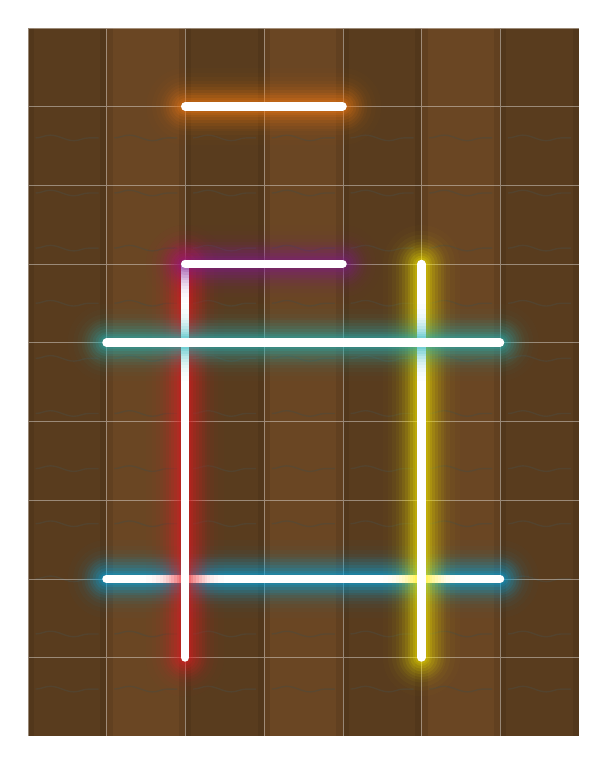
\begin{tikzpicture}[x=1cm,y=1cm]
  \def\W{7} \def\H{9}

  % ----- WOOD WALL (drawn first) -----
  \colorlet{plankA}{brown!55!black}
  \colorlet{plankB}{brown!65!black}

  % vertical planks
  \foreach \i in {0,...,\numexpr\W-1\relax} {%
    \pgfmathparse{mod(\i,2)==0?"plankA":"plankB"}\edef\col{\pgfmathresult}%
    \fill[\col!85!black] (\i,0) rectangle (\i+1,\H);
    \fill[black,opacity=0.08] (\i,0) rectangle (\i+0.08,\H);
    \fill[black,opacity=0.08] (\i+0.92,0) rectangle (\i+1,\H);
    % grain
    \foreach \y in {0.6,1.3,...,7.7} {%
      \draw[white!5!yellow!20!black, line width=0.5pt, opacity=0.5,
            decorate, decoration={snake, amplitude=0.35mm, segment length=6mm}]
        (\i+0.1,\y) -- (\i+0.9,\y);
    }%
  }%

  % grid over wood
  \begin{scope}
    \clip (0,0) rectangle (\W,\H);
    \draw[white,opacity=0.4,line width=0.1pt,step=1] (0,0) grid (\W,\H);
  \end{scope}

  % ----- YOUR NEON LINES -----
  \neonline[StallCyan]{(1,2) -- (6,2)};
  \neonline[StallRed]{(2,1) -- (2,6)};
  \neonline[StallYellow]{(5,1) -- (5,6)};
  \neonline[StallTurquoise]{(1,5) -- (6,5)};
  \neonline[StallPurple]{(2,6) -- (4,6)};
  \neonline[StallOrange]{(2,8) -- (4,8)};

  %\neonlineDistinct[StallPurple]{(6,4) -- (6,8)};
\end{tikzpicture}
\end{document}
